\subsection{Server Utilization}
\label{subsec:server_util}

During all measurements, CPU and network utilization on the server has been monitored and measured. The different results can be categorized into low latency and high latency measurements. For that reason only the server utilization for the local and North America measurements will be presented. The performance graphs for the server CPU utilization is similar to RTT and request rate graphs and shown in Figure \ref{fig:cpu}   

\begin{figure}[H]
\centering
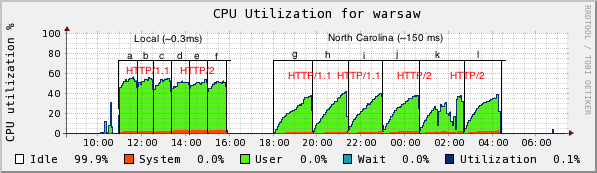
\includegraphics[scale=0.6,trim=0.0cm .0cm .0cm .0cm,clip]{images/cpu.png}
\caption{Server CPU utilization for Local and North America measurements}
\label{fig:cpu}
\end{figure}

The left part of the graph shows the CPU utilization for local measurements (from 11am - 4pm) on the server. A sudden increase up to 60\% which stays until the measurements are finished, is remarkable. That correlates to the graphs for RTT and request rates for local measurements. Starting from 6pm until 4am measurements over a high latency link (North America) were performed. We see a constant growing of the CPU graph until the maximum number of clients of 750 for each test is reached. A nearly identical characteristic shows the bandwidth utilization graph. For the measurements with larger page sizes we see more traffic flowing (Figure \ref{fig:network}.

\begin{figure}[H]
\centering
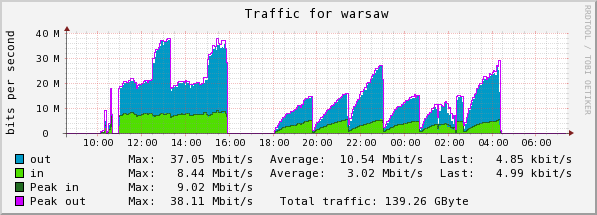
\includegraphics[scale=0.6,trim=0.0cm .0cm .0cm .0cm,clip]{images/network.png}
\caption{Server Bandwidth utilization for Local and North America measurements}
\label{fig:network}
\end{figure}

It is worth to mention that for all HTTP/1.1 measurements a lot of TCP TIME WAIT connections were discovered on the server. TCP TIME WAITS occur when the endpoint (server) blocks a current connection before it can close it due to some missing packets for that particular session. That happens because the server has much more TCP connections to manage for HTTP/1.1. The graph representing the TCP socket states on the server is shown in Figure \ref{fig:sockets}

\begin{figure}[H]
\centering
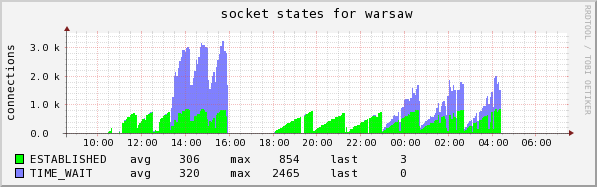
\includegraphics[scale=0.6,trim=0.0cm .0cm .0cm .0cm,clip]{images/sockets.png}
\caption{Server sockets for Local and North America measurements}
\label{fig:sockets}
\end{figure}